\chapter{Threads}

\epigraph{If you think your programs were not working before, just wait until they crash ten times as fast}{Bhuvy}

A thread is short for `thread-of-execution'.
It represents the sequence of instructions that the CPU has and will execute.
To remember how to return from function calls, and to store the values of automatic variables and parameters a thread uses a stack.
Almost weirdly, a thread is a process, meaning that creating a thread is similar to \keyword{fork}, except there is \textbf{no copying} meaning no copy on write.
What this allows is for a process to share the same address space, variables, heap, file descriptors and etc.
The actual system call to create a thread is similar to \keyword{fork}. It's \keyword{clone}.
We won't go into the specifics but you can read the \href{http://man7.org/linux/man-pages/man2/clone.2.html}{man pages} keeping in mind that it is outside the direct scope of this course.
LWP or Lightweight Processes or threads are preferred to forking for a lot of scenarios because there is a lot less overhead creating them.
But in some cases, notably python uses this, multiprocessing is the way to make your code faster.

\section{Processes vs threads}

Creating separate processes is useful when

\begin{itemize}
\item When more security is desired. For example, Chrome browser uses different processes for different tabs.
\item When running an existing and complete program then a new process is required, for example starting `gcc'.
\item When you are running into synchronization primitives and each process is operating on something in the system.
\item When you have too many threads -- the kernel tries to schedule all the threads near each other which could cause more harm than good.
\item When you don't want to worry about race conditions
\item If one thread blocks in a task (say IO) then all threads block. Processes don't have that same restriction.
\item When the amount of communication is minimal enough that simple IPC needs to be used.
\end{itemize}

On the other hand, creating threads is more useful when
\begin{itemize}
\item You want to leverage the power of a multi-core system to do one task
\item When you can't deal with the overhead of processes
\item When you want communication between the processes simplified
\item When you want to threads to be part of the same process
\end{itemize}

\section{Thread Internals}

Your main function and other functions you might call has automatic variables.
We will store them in memory using a stack and keep track of how large the stack is by using a simple pointer (the ``stack pointer'').
If the thread calls another function, we move our stack pointer down, so that we have more space for parameters and automatic variables.
Once it returns from a function, we can move the stack pointer back up to its previous value.
We keep a copy of the old stack pointer value - on the stack!
This is why returning from a function is very quick - it's easy to `free' the memory used by automatic variables - we just need to change the stack pointer.

In a multi threaded program, there are multiple stack but only one address space. The pthread library allocates some stack space and uses the \keyword{clone} function call to start the thread at that stack address.

\begin{figure}[H]
\centering
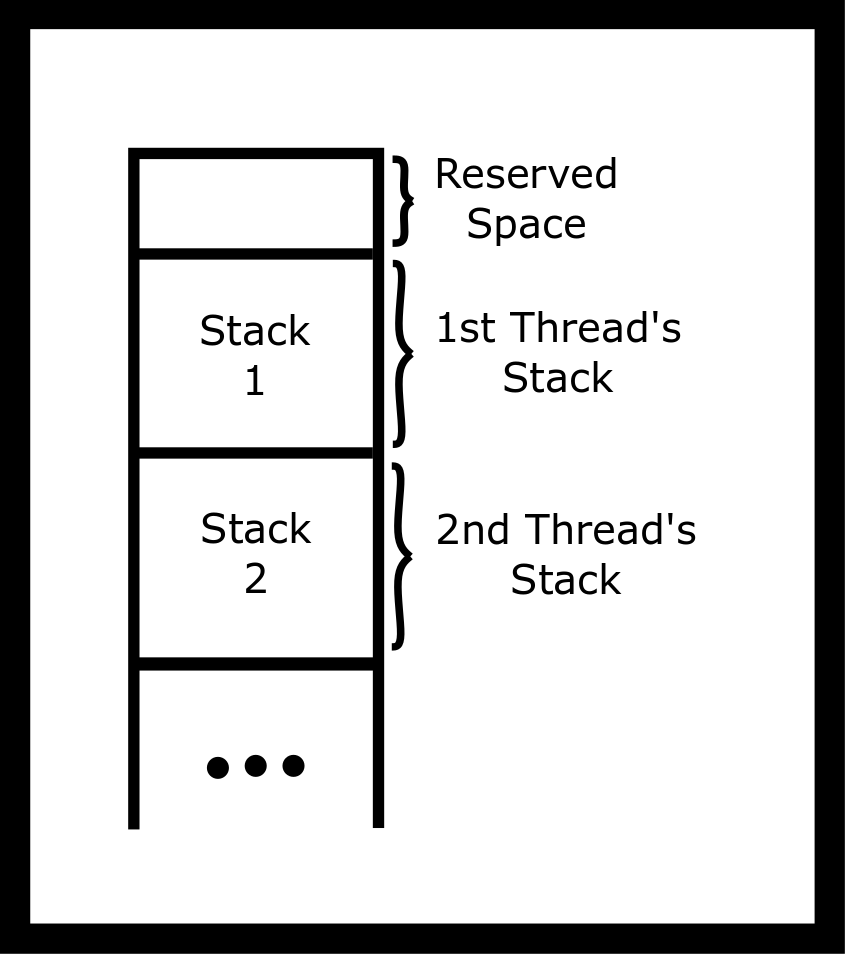
\includegraphics[width=.5\textwidth]{threads/drawings/thread_stack.png}
\caption{Thread stack visualization}
\end{figure}


You can have more than one thread running inside a process.
You get the first thread for free! It runs the code you write inside `main'.
If you need more threads you can call \keyword{pthread\_create} to create a new thread using the pthread library. You'll need to pass a pointer to a function so that the thread knows where to start.

The threads you create all live inside the same virtual memory because they are part of the same process.
Thus they can all see the heap, the global variables and the program code etc.

\begin{figure}[H]
\centering
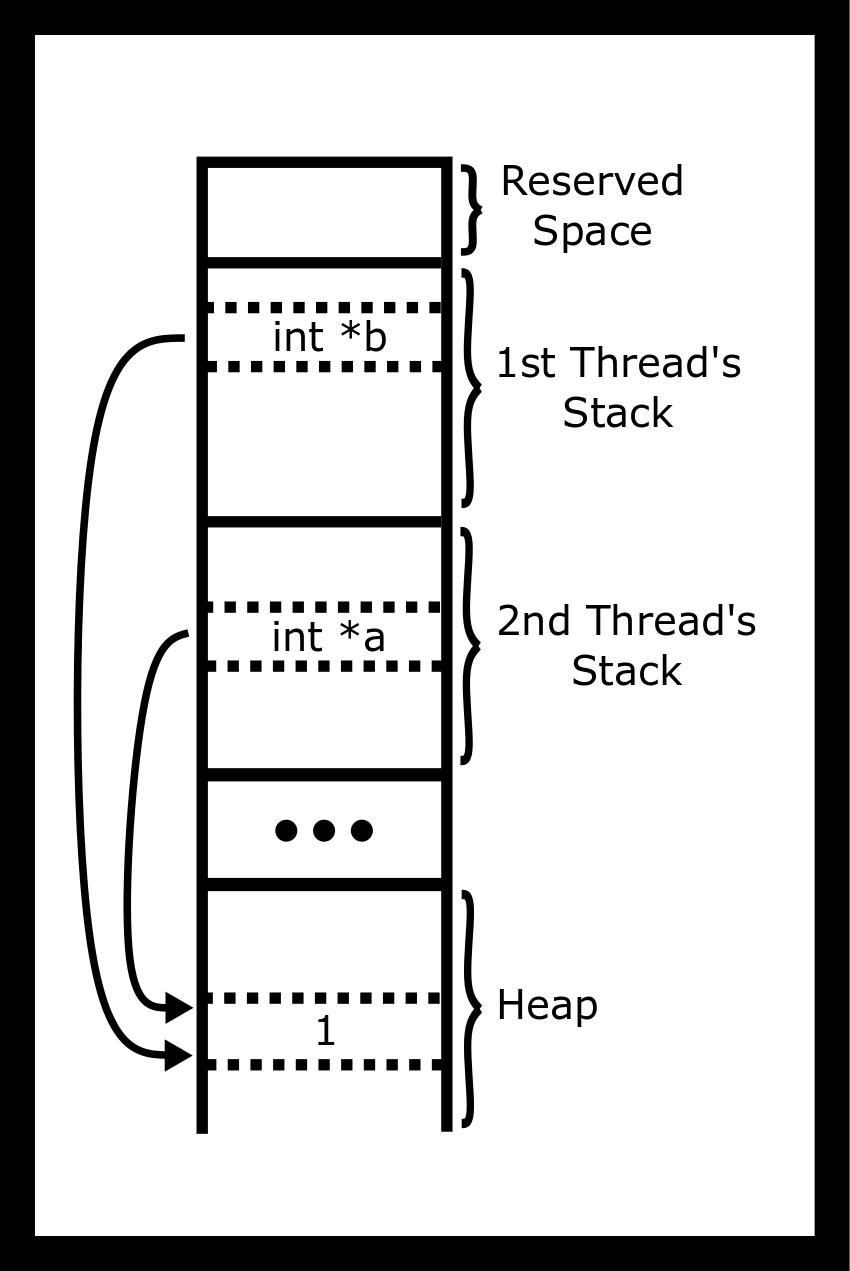
\includegraphics[width=.5\textwidth]{threads/drawings/thread_stack_pointer.png}
\caption{Threads pointing to same place in heap}
\end{figure}

Thus you can have two (or more) CPUs working on your program at the same time and inside the same process.
It's up to the operating system to assign the threads to CPUs.
If you have more active threads than CPUs, the kernel will assign the thread to a CPU for a short duration or until it runs out of things to do and then will automatically switch the CPU to work on another thread.
For example, one CPU might be processing the game AI while another thread is computing the graphics output.

\section{Simple Usage}

To use pthreads you will need to include \keyword{pthread.h} and compile and link with \keyword{-pthread} or \keyword{-lpthread} compiler option.
This option tells the compiler that your program requires threading support.
To create a thread use the function \keyword{pthread\_create}. This function takes four arguments:

\begin{lstlisting}[language=C]
int pthread_create(pthread_t *thread, const pthread_attr_t *attr,
void *(*start_routine) (void *), void *arg);
\end{lstlisting}

\begin{itemize}
\tightlist
\item
  The first is a pointer to a variable that will hold the id of the newly created thread.
\item
  The second is a pointer to attributes that we can use to tweak and tune some of the advanced features of pthreads.
\item
  The third is a pointer to a function that we want to run
\item
  Fourth is a pointer that will be given to our function
\end{itemize}

The argument \keyword{void *(*start\_routine) (void *)} is difficult to read!
It means a pointer that takes a \keyword{void *} pointer and returns a \keyword{void *} pointer.
It looks like a function declaration except that the name of the function is wrapped with \keyword{(* .... )}

\begin{lstlisting}[language=C]
#include <stdio.h>
#include <pthread.h>

void *busy(void *ptr) {
  // ptr will point to "Hi"
  puts("Hello World");
  return NULL;
}
int main() {
  pthread_t id;
  pthread_create(&id, NULL, busy, "Hi");
  void *result;
  pthread_join(id, &result);
}
\end{lstlisting}

In the above example, \keyword{result} will be \keyword{null} because the busy function returned \keyword{null}.
We need to pass the address-of result because \keyword{pthread\_join} will be writing into the contents of our pointer.

In the man pages, it warns that programmers should use \keyword{pthread\_t} as an opaque type and not look at the internals.
We do ignore that often, though.

\section{Pthread Functions}

Here are some common pthread functions to help you get going.

\begin{itemize}
\item \keyword{pthread\_create}.
Creates a new thread.
Every thread that gets created gets a new stack.
If you call \keyword{pthread\_create} twice, Your process will contain three stacks - one for each thread.
The first thread is created when the process starts, and you created two more.
Actually there can be more stacks than this, but let's keep it simple.
The important idea is that each thread requires a stack because the stack contains automatic variables and the old CPU PC register, so that it can go back to executing the calling function after the function is finished.

\item \keyword{pthread\_cancel} stops a thread.
Note the thread may not actually be stopped immediately.
For example it can be terminated when the thread makes an operating system call (e.g. \keyword{write}).
In practice, \keyword{pthread\_cancel} is rarely used because it does not give a thread an opportunity to clean up after itself (for example, it may have opened some files).
An alternative implementation is to use a boolean (int) variable whose value is used to inform other threads that they should finish and clean up.

\item \keyword{pthread\_exit(void *)} stops the calling thread meaning the thread never returns after calling \keyword{pthread\_exit}.
The pthread library will automatically finish the process if there are no other threads running.
\keyword{pthread\_exit(...)} is equivalent to returning from the thread's function; both finish the thread and also set the return value (void *pointer) for the thread.
Calling \keyword{pthread\_exit} in the \keyword{main} thread is a common way for simple programs to ensure that all threads finish.
For example, in the following program, the \keyword{myfunc} threads will probably not have time to get started.
On the other hand \keyword{exit()} exits the entire process and sets the process' exit value.
This is equivalent to \keyword{return ();} in the main method.
All threads inside the process are stopped.
Note the \keyword{pthread\_exit} version creates thread zombies, however this is not a long-running process, so we don't care.

\begin{lstlisting}[language=C]
int main() {
  pthread_t tid1, tid2;
  pthread_create(&tid1, NULL, myfunc, "Jabberwocky");
  pthread_create(&tid2, NULL, myfunc, "Vorpel");
  if (keep_threads_going) {
    pthread_exit(NULL);
  } else {
    exit(42); //or return 42;
  }

  // No code is run after exit
}
\end{lstlisting}

\item \keyword{pthread\_join()} waits for a thread to finish and records its return value.
Finished threads will continue to consume resources.
Eventually, if enough threads are created, \keyword{pthread\_create} will fail.
In practice, this is only an issue for long-running processes but is not an issue for simple, short-lived processes as all thread resources are automatically freed when the process exits.
This is equivalent to turning your children into zombies, so keep this in mind for long running processes. In the exit example, we could also wait on all the threads.

\begin{lstlisting}[language=C]
// ...
void* result;
pthread_join(tid1, &result);
pthread_join(tid2, &result);
return 42;
// ...
\end{lstlisting}


\end{itemize}

There are many ways to exit threads.
Here is a non-complete list.

\begin{itemize}
\item Returning from the thread function
\item Calling \keyword{pthread\_exit}
\item Cancelling the thread with \keyword{pthread\_cancel}
\item Terminating the process through a signal.
\item calling \keyword{exit()} or \keyword{abort()}
\item Returning from \keyword{main}
\item \keyword{exec}'ing another program
\item Unplugging your computer
\item Some undefined behavior can terminate your threads, it is undefined behavior
\end{itemize}

\section{Race Conditions}

Race conditions are whenever the outcome of a program is determined by its sequence of events determined by the processor.
This means that the execution of the code is non-deterministic.
Meaning that the same program can run multiple times and depending on how the kernel schedules the threads could produce inaccurate results.
The following is the canonical race condition.

\begin{lstlisting}[language=C]
void *thread_main(void *p) {
  int x = *p;
  x += x;
  *p = x;
  return NULL;
}

int main() {
  int data = 1;
  pthread_t one, two;
  pthread_create(&one, NULL, thread_main, &data);
  pthread_create(&two, NULL, thread_main, &data);
  pthread_join(one, NULL);
  pthread_join(two, NULL);
  printf("%d\n", data);
  return 0;
}
\end{lstlisting}

Breaking down the assembly there are many different accesses of the code.
We will assume that data is stored in the \keyword{eax} register.
The code to increment is the following with no optimization (assume int\_ptr contains eax).

\begin{lstlisting}[language={[x86masm]Assembler}]
mov eax, DWORD PTR [rbp-4]    ;Loads int_ptr
add eax, eax                  ;Does the addition
mov DWORD PTR [rbp-4], eax    ;Stores it back
\end{lstlisting}

Consider this access pattern.

\begin{figure}[H]
\centering
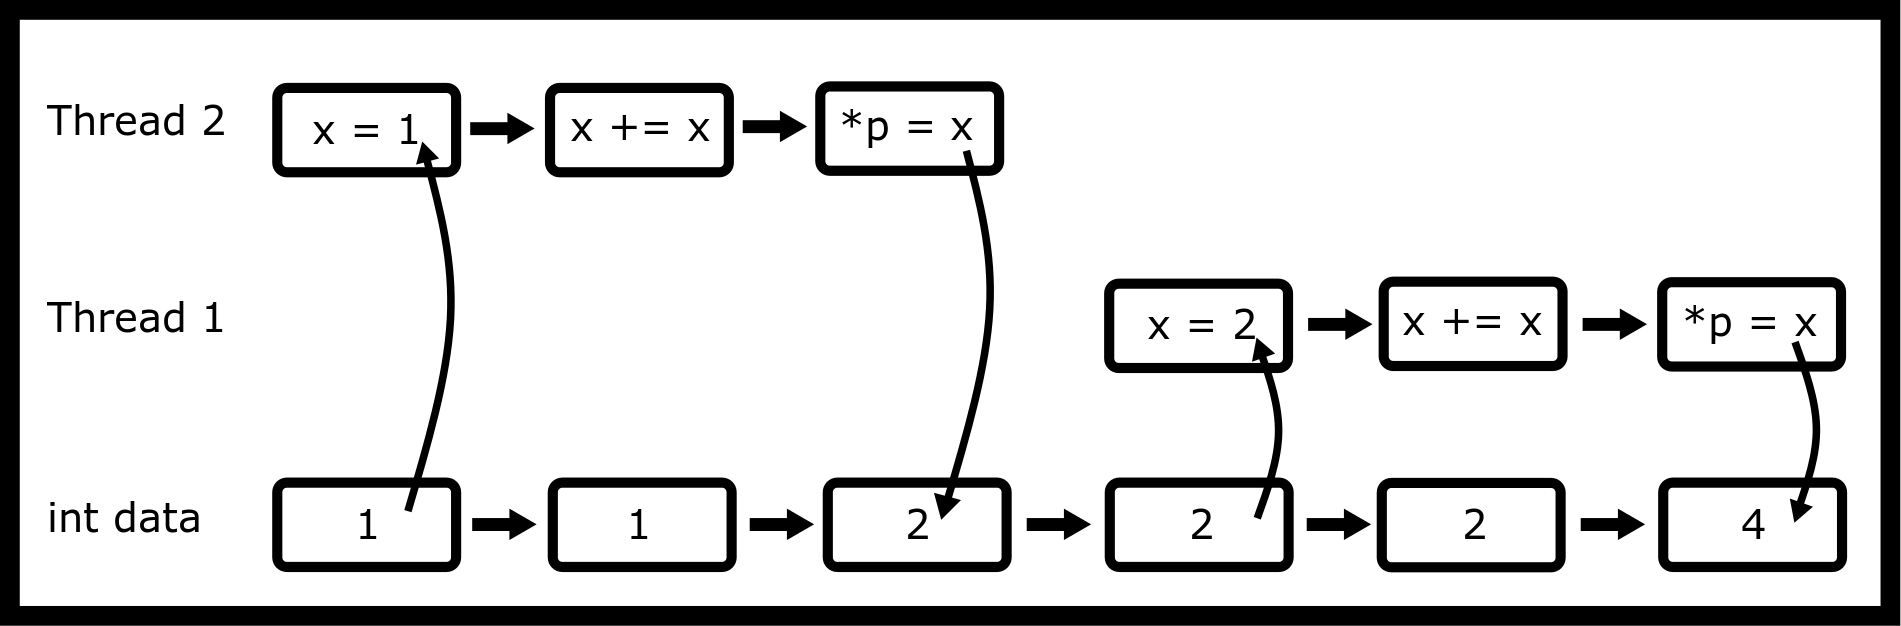
\includegraphics[width=.7\textwidth]{threads/drawings/thread_nonrace_timing.png}
\caption{Thread access - not a race condition}
\end{figure}

This access pattern will cause the variable \keyword{data} to be 4.
The problem is when the instructions are executed in parallel.

\begin{figure}[H]
\centering
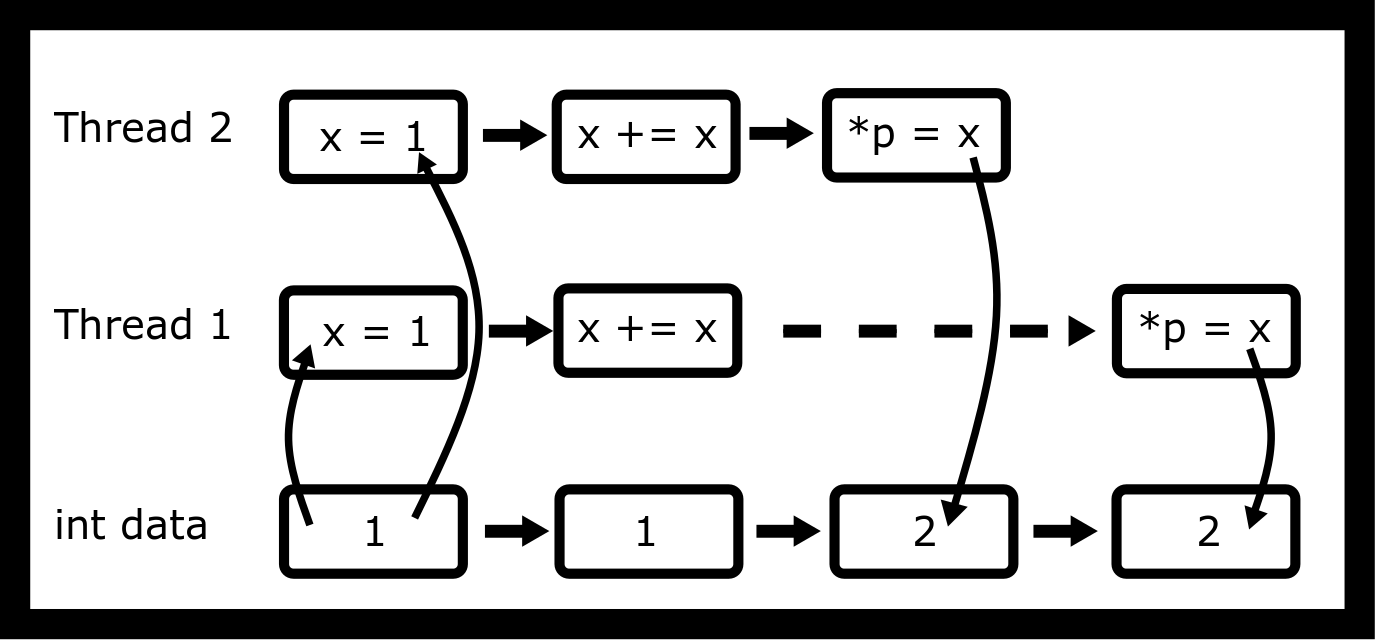
\includegraphics[width=.5\textwidth]{threads/drawings/thread_race_timing.png}
\caption{Thread access - race condition}
\end{figure}

This access pattern will cause the variable \keyword{data} to be 2.
This is undefined behavior and a race condition.
What we want is one thread to access the part of the code at a time.

You may also ask, well when I compile the code with \keyword{-O2} then I get

\begin{lstlisting}[language={[x86masm]Assembler}]
shl dword ptr [rdi]   # Optimized way of doing the add
\end{lstlisting}

Shouldn't that fix it? It is a single assembly instructions so no interleaving?
Well it doesn't fix the problems that the \textit{hardware itself} may experience a race condition because we as programmers didn't tell the hardware to check for it.
The easiest way is to add the \textit{lock} prefix \cite[p. 1120]{guide2011intel}.

But we don't want to be coding in assembly!
We need to come up with a software solution to this problem.

\subsubsection{A day at the races}

Here is another small race condition.
The following code is supposed to start ten threads with the integers 0 through 9 inclusive.
However, when run prints out \keyword{1 7 8 8 8 8 8 8 8 10}!
Or very seldom does it print out what we expect.
Can you see why?

\begin{lstlisting}[language=C]
#include <pthread.h>
void* myfunc(void* ptr) {
  int i = *((int *) ptr);
  printf("%d ", i);
  return NULL;
}

int main() {
  // Each thread gets a different value of i to process
  int i;
  pthread_t tid;
  for(i =0; i < 10; i++) {
    pthread_create(&tid, NULL, myfunc, &i); // ERROR
  }
  pthread_exit(NULL);
}
\end{lstlisting}

The above code suffers from a \keyword{race condition} - the value of i is changing.
The new threads start later in the example output the last thread starts after the loop has finished.
To overcome this race-condition, we will give each thread a pointer to its own data area.
For example, for each thread we may want to store the id, a starting value and an output value.
We will instead treat i as a pointer and cast it by value.

\begin{lstlisting}[language=C]
void* myfunc(void* ptr) {
  int data = ((int) ptr);
  printf("%d ", data);
  return NULL;
}

int main() {
  // Each thread gets a different value of i to process
  int i;
  pthread_t tid;
  for(i =0; i < 10; i++) {
    pthread_create(&tid, NULL, myfunc, (void *)i);
  }
  pthread_exit(NULL);
}
\end{lstlisting}

Race conditions aren't just in our code.
they can be in provided code
Some functions like \keyword{asctime}, \keyword{getenv}, \keyword{strtok}, \keyword{strerror} not thread-safe.
Let's look at a simple function that is also not `thread-safe'.
The result buffer could be stored in global memory.
This is good in a single threaded program.
We wouldn't want to return a pointer to an invalid address on the stack, but there's only one result buffer in the entire memory.
If two threads were to use it at the same time, one would corrupt the other.

\begin{lstlisting}[language=C]
char *to_message(int num) {
  static char result [256];
  if (num < 10) sprintf(result, "%d : blah blah" , num);
  else strcpy(result, "Unknown");
  return result;
}
\end{lstlisting}

There are ways around this like using synchronization locks, but first let's do this by design.
How would you fix the function above?
You can change any of the parameters and any return types.
Here is one valid solution.

\begin{lstlisting}[language=C]
int to_message_r(int num, char *buf, size_t nbytes) {
  size_t written;
  if (num < 10) {
    written = snprintf(buf, nbtytes, "%d : blah blah" , num);
  } else {
    strncpy(buf, "Unknown", nbytes);
    buf[nbytes] = '\0';
    written = strlen(buf) + 1;
  }
  return written <= nbytes;
}
\end{lstlisting}

Instead of making the function responsible for the memory, we made the caller responsible!
A lot of programs, and hopefully your programs, have minimal communication needed.
Often a malloc call is much less work than locking a mutex or sending a message to another thread.

\subsection{Don't Cross the Streams}

In case you were wondering, you can fork inside a process with multiple threads!
However, the child process only has a single thread, which is a clone of the thread that called \keyword{fork}.
We can see this as a simple example, where the background threads never print out a second message in the child process.

\begin{lstlisting}[language=C]
#include <pthread.h>
#include <stdio.h>
#include <unistd.h>

static pid_t child = -2;

void *sleepnprint(void *arg) {
  printf("%d:%s starting up...\n", getpid(), (char *) arg);

  while (child == -2) {sleep(1);} /* Later we will use condition variables */

  printf("%d:%s finishing...\n",getpid(), (char*)arg);

  return NULL;
}
int main() {
  pthread_t tid1, tid2;
  pthread_create(&tid1,NULL, sleepnprint, "New Thread One");
  pthread_create(&tid2,NULL, sleepnprint, "New Thread Two");

  child = fork();
  printf("%d:%s\n",getpid(), "fork()ing complete");
  sleep(3);

  printf("%d:%s\n",getpid(), "Main thread finished");

  pthread_exit(NULL);
  return 0; /* Never executes */
}
\end{lstlisting}

\begin{verbatim}
8970:New Thread One starting up...
8970:fork()ing complete
8973:fork()ing complete
8970:New Thread Two starting up...
8970:New Thread Two finishing...
8970:New Thread One finishing...
8970:Main thread finished
8973:Main thread finished
\end{verbatim}

In practice, creating threads before forking can lead to unexpected errors because (as demonstrated above) the other threads are immediately terminated when forking.
Another thread might have just lock a mutex like by calling malloc and never unlock it again.
Advanced users may find \keyword{pthread\_atfork} useful however we suggest you usually try to avoid creating threads before forking unless you fully understand the limitations and difficulties of this approach.

\subsection{Embarrassingly Parallel Problems}

The study of parallel algorithms has exploded over the past few years.
An embarrassingly parallel problem is any problem that needs little effort to turn parallel.
A lot of them have some synchronization concepts with them but not always.
You already know a parallelizable algorithm, Merge Sort!

\begin{lstlisting}[language=C]
void merge_sort(int *arr, size_t len){
  if(len > 1){
    // Merge Sort the left half
    // Merge Sort the right half
    // Merge the two halves
  }
\end{lstlisting}

With your new understanding of threads, all you need to do is create a thread for the left half, and one for the right half.
Given that your CPU has multiple real cores, you will see a speedup in accordance with \href{https://en.wikipedia.org/wiki/Amdahl's_law}{Amdahl's Law}.
The time complexity analysis gets interesting here as well.
The parallel algorithm runs in $O(\log^3(n))$ running time because we have the analysis assumes that we have a lot of cores.

In practice though, we typically do two changes.
One, once the array gets small enough, we ditch the parallel Merge Sort algorithm and do a quicksort or other algorithm that works fast on small arrays, usually cache coherency rules at this level.
The other thing that we know is that CPUs don't have infinite cores.
To get around that, we typically keep a worker pool.
You won't see the speedup right away because of things like cache coherency and scheduling extra threads.
Over the long term though, you will start to see speedups.

Another embarrassingly parallel problem is parallel map.
Say we want to apply a function to an entire array, one element at a time.

\begin{lstlisting}[language=C]
int *map(int (*func)(int), int *arr, size_t len){
  int *ret = malloc(len*sizeof(*arr));
  for(size_t i = 0; i < len; ++i) {
    ret[i] = func(arr[i]);
  }
  return ret;
}
\end{lstlisting}

Since none of the elements depend on any other element, how would you go about parallelizing this?
What do you think would be the best way to split up the work between threads.

\subsection{Extra: Scheduling}

There are a few ways to split up the work.
These are common to the OpenMP framework \cite{silberschatz2005operating}.

\begin{itemize}
\item \keyword{static scheduling} break up the problems into fixed size chunks (predetermined) and have each thread work on each of the chunks.
  This works well when each of the subproblems take roughly the same time because there is no additional overhead.
  All you need to do is write a loop and give the map function to each sub-array.
\item \keyword{dynamic scheduling} as a new problem becomes available have a thread serve it.
  This is useful when you don't know how long the scheduling will take
\item \keyword{guided scheduling} This is a mix of the above with a mix of the benefits and tradeoffs.
  You start with a static scheduling and move slowly to dynamic if needed
\item \keyword{runtime scheduling} You have absolutely no idea how long the problems are going to take.
  Instead of deciding it yourself, let the program decide what to do!
\end{itemize}

No need to memorize any of the scheduling routines though.
Openmp is a standard that is an alternative to pthreads.
For example here is how to parallelize a for loop

\begin{lstlisting}[language=C]
#pragma omp parallel for
for (int i = 0; i < n; i++) {
  // Do stuff
}

// Specify the scheduling as follows
// #pragma omp parallel for scheduling(static)
\end{lstlisting}

Static scheduling will divide the problem into fixed size chunks
Dynamic scheduling will give a job once the loop is over
Guided scheduling is Dynamic with chunks
Runtime is a whole bag of worms.

\subsection{Other Problems}

From \href{https://en.wikipedia.org/wiki/Embarrassingly_parallel}{Wikipedia}
\begin{itemize}
\tightlist
\item Serving static files on a web server to multiple users at once.
\item The Mandelbrot set, Perlin noise and similar images, where each point is calculated independently.
\item Rendering of computer graphics. In computer animation, each frame may be rendered independently (see parallel rendering).
\item Brute-force searches in cryptography.
\item Notable real-world examples include distributed.net and proof-of-work systems used in cryptocurrency.
\item BLAST searches in bioinformatics for multiple queries (but not for individual large queries)
\item Large scale facial recognition systems that compare thousands of arbitrary acquired faces (e.g., a security or surveillance video via closed-circuit television) with similarly large number of previously stored faces (e.g., a rogues gallery or similar watch list).
\item Computer simulations comparing many independent scenarios, such as climate models.
\item Evolutionary computation meta-heuristics such as genetic algorithms.
\item Ensemble calculations of numerical weather prediction.
\item Event simulation and reconstruction in particle physics.
\item The marching squares algorithm
\item Sieving step of the quadratic sieve and the number field sieve.
\item Tree growth step of the random forest machine learning technique.
\item Discrete Fourier Transform where each harmonic is independently calculated.
\end{itemize}

\subsection{Extra: threads.h}

We have a lot of threading libraries discussed in the extra section.
We have the standard POSIX threads, OpenMP threads, we also have a new C11 threading library that is built into the standard.
This library provides restricted functionality.

You ask yourself, why would I use the restricted functionality?
The key is in the name.
Since this is the C standard library, it has to be implemented on all operating systems that are compliant which are pretty much all of them.
This means there is first-class portability when using threads.

We won't drone on about the functions.
Most of them are just renaming of pthread functions anyway.
If you ask why we don't teach these, there are a few reasons

\begin{enumerate}
\item They are pretty new. Even though the standard came out in roughly 2011, POSIX threads have been around forever.
  A lot of their quirks have been ironed out.
\item You lose expressivity.
  This is a concept that we'll talk about in layer chapters, but when you make something portable, you lose some expressivity with the host hardware.
  That means that the threads.h library is pretty bare bones.
  It is hard to set CPU affinities.
  Schedule threads together.
  Efficiently look at the internals for performance reasons.
\item A lot of legacy code is already written with POSIX threads in mind.
  Other libraries like OpenMP, CUDA, MPI will either use POSIX processes or POSIX threads with a begrudging port to Windows.
\end{enumerate}

\subsection{Extra: Lightweight Processes?}

Earlier in the beginning of the chapter we mentioned that threads are just processes.
What do we mean by that?
You can create a thread just like a process
Take a look at the example code below

\begin{lstlisting}[language=C]

// 8 KiB stacks
#define STACK_SIZE (8 * 1024 * 1024)

int thread_start(void *arg) {
  // Just like the pthread function
  puts("Hello Clone!")
  // I share the same heap and address space!
  return 0;
}

int main() {
  // Allocate stack space for the child
  char *child_stack = malloc(STACK_SIZE);
  // Remember stacks work by growing down, so we need
  // to give the top of the stack
  char *stack_top = stack + STACK_SIZE;

  // clone create thread
  pid_t pid = clone(thread_start, stack_top, SIGCHLD, NULL);
  if (pid == -1) {
    perror("clone");
    exit(1);
  }
  printf("Child pid %ld\n", (long) pid);

  // Wait just like any child
  if (waitpid(pid, NULL, 0) == -1) {
    perror("waitpid");
    exit(1);
  }

  return 0;
}
\end{lstlisting}

Seems pretty simple right?
Well why don't we have you do it this way every time?
First there is a decent bit of boilerplate code.
You have to create the stack every time and pass in the right flags, and wait like a process which requires a lot of finicky flags to be set from the man pages.
In addition, almost everyone uses pthreads by default.
Pthreads let you set various attributes -- some that resemble the option in clone -- to customize your thread.
But as we mentioned earlier, with each later of abstraction for portability reasons we lose some functionality.
clone can do some neat things like keep different parts of your heap the same while creating copies of other pages.
You have finer linux control of scheduling because it is a process, just with the same mappings.

At no time in this course should you be using clone.
But in the future, know that it is a perfectly viable alternative to fork.
You just have to be careful about what you are doing.

\subsection{Further Reading}

\begin{itemize}
\item \href{http://man7.org/linux/man-pages/man3/pthread_create.3.html}{man page}
\item \href{http://man7.org/linux/man-pages/man7/pthreads.7.html}{pthread reference guide}
\item \href{http://www.thegeekstuff.com/2012/04/terminate-c-thread/}{Concise third party sample code explaining create, join and exit}
\end{itemize}

\section{Topics}

\begin{itemize}
\tightlist
\item
pthread life-cycle
\item
Each thread has a stack
\item
Capturing return values from a thread
\item
Using \keyword{pthread\_join}
\item
Using \keyword{pthread\_create}
\item
Using \keyword{pthread\_exit}
\item
Under what conditions will a process exit
\end{itemize}

\section{Questions}

\begin{itemize}
\tightlist
\item
What happens when a pthread gets created?
\item
Where is each thread's stack?
\item
How do you get a return value given a \keyword{pthread\_t}? What are the ways a thread can set that return value? What happens if you discard the return value?
\item
Why is \keyword{pthread\_join} important (think stack space, registers, return values)?
\item
What does \keyword{pthread\_exit} do under normal circumstances (i.e. you are not the last thread)? What other functions are called when you call pthread\_exit?
\item
Give me three conditions under which a multithreaded process will exit. Can you think of any more?
\item
What is an embarrassingly parallel problem?
\end{itemize}

\bibliographystyle{plainnat}
\bibliography{threads/threads}
